\begin{savequote}[45mm]
\ascii{Any fool can write code that a computer can understand. Good programmers write code that humans can understand.}
\qauthor{\ascii{- Martin Flower}}
\end{savequote}

\chapter{破冰之旅} 
\label{ch:ice-breaker}

\begin{content}

本章将开启\ascii{xUnit Mars}开发之旅。首先,构建\ascii{xUnit Mars}项目的开发环境,包括物理组织,构建系统,代码仓库,集成开发环境。然后,重点描述第一个测试用例诞生的全过程,体验\ascii{TDD}的开发节奏,透视设计权衡的细节之处。

% 鉴别设计的坏味道,通过重构得到简单设计,这就是软件设计内在的美感。犹如遇到一件困难的事情,采用最简单的方法,漂亮地攻克了这个问题,这种成就感油然而生。优美的设计,简单的实现,是所有程序员梦寐追求的目标之一。

\end{content}

\section{编程环境}

\begin{content}

\ascii{xUnit Mars}采用现代风格的\cpp{}语言实现。\cpp{}是一门极其复杂的程序设计语言,拥有强悍的抽象能力与设计工具,但也存在众多瑕疵为人所诟病。

我们会尽最大可能地使用语言的优秀特性,去其糟粕,取其精华。我们不推崇故弄玄虚,奇技淫巧的价值观与方法论。关注问题与软件设计本身,是我们讨论的重点,甚至与语言实现无关。

\subsection{系统配置}

\begin{colortable}{X|X|X}{环境配置}
\emph{名称}                      & \emph{配置}          & \emph{版本}      \\\hline
\multirow{2}{*}\ascii{操作系统}  & \ascii{Linux Kernel} & \ascii{4.15.0}  \\\cline{2-3}
                                & \ascii{Ubuntu}       & \ascii{18.04}   \\\hline
\multirow{2}{*}\ascii{编译器}    & \ascii{GCC}          & \ascii{7.3.0}   \\\cline{2-3}
                                & \ascii{Clang}        & \ascii{6.0.0}   \\\hline
\ascii{编程语言} & \ascii{C++}   & \ascii{14}                              \\\hline
\multirow{2}{*}\ascii{构建工具}  & \ascii{CMake}        & \ascii{3.10}     \\\cline{2-3} 
                                & \ascii{Make}         & \ascii{4.10}     \\\hline
\ascii{集成开发环境}              & \ascii{Eclipse CDT}  & \ascii{Oxygen 3} \\\hline 
\ascii{版本工具}                 & \ascii{Git}          & \ascii{2.17.1}   \\\hline
\end{colortable}

\subsection{项目组织}

项目\ascii{xUnit Mars}物理目录如\refig{mars-project}所示。此处将头文件,实现文件,测试文件相分离,纯属个人偏好。我也很推崇\ascii{Google}风格,将头文件,实现文件,测试文件放一起,易于工程管理。

\begin{figure}[H]
\centering
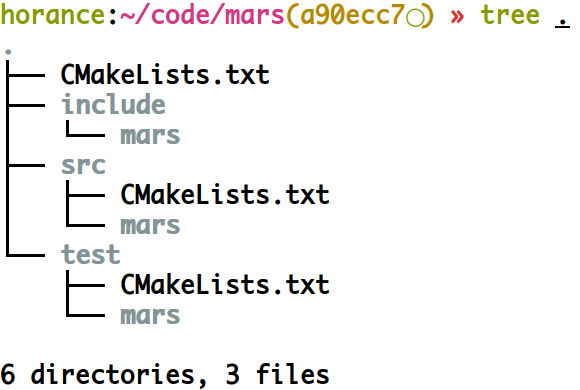
\includegraphics[width=0.6\textwidth]{figures/xunit/mars-project.png}
\caption{xUnit Mars: 项目组织}
 \label{fig:mars-project}
\end{figure}

\subsection{构建系统}

\ascii{xUnit Mars}使用\ascii{CMake}构建工具。在项目根目录下,主控\ascii{CMakeLists.txt}完成项目的整体配置,及其子任务的组织。

\begin{nodiff}{CMakeLists.txt}
 \begin{c++}
project(mars)                                                                                  
cmake_minimum_required(VERSION 2.8)

set(CMAKE_CXX_FLAGS "${CMAKE_CXX_FLAGS} -std=c++14")

include_directories("${CMAKE_CURRENT_SOURCE_DIR}/include")

add_subdirectory(src)
add_subdirectory(test)
 \end{c++}
\end{nodiff}

\ascii{src/CMakeLists.txt}完成\ascii{mars}库构建。

\begin{nodiff}{src/CMakeLists.txt}
 \begin{c++}
file(GLOB_RECURSE all_files *.cc)
add_library(mars STATIC ${all_files})
 \end{c++}
\end{nodiff}

\ascii{test/CMakeLists.txt}完成\ascii{mars-test}应用程序构建,它执行\ascii{xUnit Mars}项目的所有测试用例。

\begin{nodiff}{test/CMakeLists.txt}
 \begin{c++}
file(GLOB_RECURSE all_files *.cc)
add_executable(mars-test ${all_files})
target_link_libraries(mars-test mars gtest gtest_main pthread)
 \end{c++}
\end{nodiff}

\subsection{Git库}

在项目根目录下初始化一个空的\ascii{Git}库。

\begin{nodiff}{初始化git库}
 \begin{c++}
$ git init
 \end{c++}
\end{nodiff}  

待项目组织完毕,完成第一次代码提交。

\begin{nodiff}{提交代码}
 \begin{c++}
$ git add -A .
$ git commit -m"setup cmake project"
 \end{c++}
\end{nodiff}

\end{content}

\section{伊始}

\begin{content}

万事开头难,说得没错。但更重要的是,要努力让事情一开始就是对的。学习如此,生活亦如此,凡事大抵莫能例外。关键如何知道自己就是对的那个人呢?反馈,是一种有效的信息传递机制。刺激变化,让测试尽早模拟客户现场,并挖掘潜在的抽象。

\subsection{初出茅庐}

但是,将第一个测试用例跑起来并不容易。这里尝试模拟设计一个\ascii{xUnit Mars}风格的测试用例,将其命名为\ascii{WasRun},它包含了一个\emph{测试方法}:\ascii{WasRun::testMethod}。当测试方法\ascii{WasRun::testMethod}被执行后,断言其状态与行为是否符合预期。

\begin{nodiff}{test/mars/core/TestMethodSpec.cc}
\begin{c++}
#include <gtest/gtest.h>

namespace {
  struct WasRun {
    bool wasRun = false;

    void testMethod() {
      wasRun = true;
    }
  };
}

TEST(WasRunSpec, make_sure_test_method_be_ran) {
  WasRun test;

  ASSERT_FALSE(test.wasRun);
  test.testMethod();
  ASSERT_TRUE(test.wasRun);
}
\end{c++}
\end{nodiff}

但是这个测试很鸡肋,不仅天然地通过,而且不能驱动出任何的产品代码。仔细思量,\ascii{xUnit Mars}引擎主要负责组织、调度和执行测试用例,它应该对外开放执行\emph{测试方法}的\ascii{API}。而\ascii{testMethod}是\ascii{WasRun}的一个成员函数,除了可以通过\code{test.testMethod}实现\emph{直接调用}之外,还可以通过指向成员函数的指针实现\emph{间接调用}。其中,后者须具备两个基本条件:

\begin{enum}
  \eitem{测试对象:\code{WasRun}实例;}
  \eitem{测试方法:指向成员函数\code{WasRun::testMethod}的指针。}
\end{enum}

\subsubsection{零号用例}

据此,引入\ascii{xUnit Mars}执行测试方法的核心\ascii{API}:\ascii{run}函数。其第一个参数接受\ascii{WasRun}的测试对象,第二个参数接受指向成员函数\ascii{WasRun::testMethod}的指针。相比之前的测试用例,该测试用例可以驱动出部分实现,虽然进步甚微,但已迈出具有实质意义的第一步。

\begin{diff}{test/mars/core/TestMethodSpec.cc}
\begin{minicpp}
#include <gtest/gtest.h>

namespace {
  struct WasRun {
    bool wasRun = false;

    void testMethod() {
      wasRun = true;
    }
  };
}

TEST(WasRunSpec, make_sure_test_method_be_ran) {
  WasRun test;

  ASSERT_FALSE(test.wasRun);
  test.testMethod();
  ASSERT_TRUE(test.wasRun);
}
\end{minicpp}
\tcblower
\begin{minicpp}
#include <gtest/gtest.h>

namespace {
  struct WasRun {
    bool wasRun = false;

    void testMethod() {
      wasRun = true;
    }
  };
}

TEST(WasRunSpec, make_sure_test_method_be_ran) {
  WasRun test;

  ASSERT_FALSE(test.wasRun);
  run(test, &WasRun::testMethod);
  ASSERT_TRUE(test.wasRun);
}
\end{minicpp}
\end{diff}

\subsubsection{通过测试}

不幸的是,\ascii{run}函数依赖于具体类型\ascii{WasRun},而\ascii{WarRun}存在于匿名命名空间内。我们不期望将\ascii{WasRun}搬迁至产品实现中,毕竟\ascii{WarRun}是一个用户自定义的测试用例。

在不破坏匿名命名空间的封装性,且不将测试代码污染产品代码的前提之下,为了快速通过测试用例,姑且就近实现\ascii{run}函数。

\begin{diff}{test/mars/core/TestMethodSpec.cc}
\begin{minicpp}
#include <gtest/gtest.h>

namespace {
  struct WasRun {
    bool wasRun = false;

    void testMethod() {
      wasRun = true;
    }
  };
}

TEST(WasRunSpec, make_sure_test_method_be_ran) {
  WasRun test;

  ASSERT_FALSE(test.wasRun);
  run(test, &WasRun::testMethod);
  ASSERT_TRUE(test.wasRun);
}
\end{minicpp}
\tcblower
\begin{minicpp}
#include <gtest/gtest.h>

namespace {
  struct WasRun {
    bool wasRun = false;

    void testMethod() {
      wasRun = true;
    }
  };

  void run(WasRun& self, void(WasRun::*method)()) {
    (self.*method)();
  }
}

TEST(WasRunSpec, make_sure_test_method_be_ran) {
  WasRun test;
  ASSERT_FALSE(test.wasRun);

  run(test, &WasRun::testMethod);
  ASSERT_TRUE(test.wasRun);
}
\end{minicpp}
\end{diff}

\subsubsection{执行测试}

在\ascii{build}临时目录中,使用\ascii{cmake}构建工程。

\begin{nodiff}{构建工程}
 \begin{c++}
$ mkdir -p build && cd build
$ cmake ..
$ make
 \end{c++}
\end{nodiff}

运行测试。

\begin{nodiff}{运行测试}
 \begin{c++}
$ test/mars-test
Running main() from gtest_main.cc
[==========] Running 1 test from 1 test case.
[----------] Global test environment set-up.
[----------] 1 test from SimpleTest
[ RUN      ] SimpleTest.make_sure_test_case_can_run_normally
[       OK ] SimpleTest.make_sure_test_case_can_run_normally (0 ms)
[----------] 1 test from SimpleTest (0 ms total)

[----------] Global test environment tear-down
[==========] 1 test from 1 test case ran. (0 ms total)
[  PASSED  ] 1 test.
 \end{c++}
\end{nodiff}

\subsubsection{提交代码}

每当通过测试后,立即提交代码到\ascii{Git}库。

\begin{nodiff}{提交代码}
 \begin{c++}
$ git add -A .
$ git commit -m"pass first test case"
 \end{c++}
\end{nodiff}

\begin{episode}{全局忽略模式}
\begin{content}

\ascii{CMake}在临时目录\ascii{build}中完成系统构建,为了避免不经意地将\ascii{build}目录提交至\ascii{Git}库,常常需要在\ascii{.gitignore}文件中配置相应的忽略模式。

但是,为每个项目都创建一个\ascii{.gitignore}文件,显然是一种重复设计。因此,配置全局忽略模式是一个更恰当的解决方案。

 \begin{c++}
$ git config --global core.excludesfile ~/.gitignore_global
$ vi ~/.gitignore_global
# cmake
build/

# vi
*.swp

# eclipse
.project
.cproject
.settings/

# tex
output/
 \end{c++}

\end{content}
\end{episode}

\subsection{引入泛型}

设计的坏味道非常明显,\ascii{run}函数与\ascii{WasRun}类型强度耦合,不够泛化。不仅无法搬迁\ascii{run}函数到产品代码中,而且不易被其他测试用例复用。新增测试用例\ascii{WasSucc}时,不得不再次重复实现\ascii{run}函数的基本逻辑。

\begin{nodiff}{test/mars/core/TestMethodSpec.cc}
\begin{c++}
#include <gtest/gtest.h>

namespace {
  struct WasRun {
    bool wasRun = false;

    void testMethod() {
      wasRun = true;
    }
  };
  
  // Duplication!!!
  void run(WasRun& self, void(WasRun::*method)()) {
    (self.*method)();
  }
}

TEST(WasRunSpec, make_sure_test_method_be_ran) {
  WasRun test;

  ASSERT_FALSE(test.wasRun);
  run(test, &WasRun::testMethod);
  ASSERT_TRUE(test.wasRun);
}

namespace {
  struct WasSucc {
    std::string result = "failed";

    void testMethod() {
      result = "success";
    }
  };

  // Duplication!!!
  void run(WasSucc& self, void(WasSucc::*method)()) {
    (self.*method)();
  }
}

TEST(WasSuccSpec, make_sure_test_method_be_ran) {
  WasSucc test;

  ASSERT_EQ("failed", test.result);
  run(test, &WasSucc::testMethod);
  ASSERT_EQ("success", test.result);
}
\end{c++}
\end{nodiff}

虽然两个测试用例是通过的,但两个特化实现的\ascii{run}函数引入了明显的重复设计。为了消除两者实现的重复设计,提取公共的模板函数\ascii{run},并搬迁至产品文件\ascii{TestMethod.h}之中。

\begin{nodiff}{include/mars/core/TestMethod.h}
\begin{c++}
#ifndef HD3E38C9A_3B03_48CE_9A1B_75B41CB012C6
#define HD3E38C9A_3B03_48CE_9A1B_75B41CB012C6

template <typename Fixture>
void run(Fixture& self, void(Fixture::*method)()) {
  (self.*method)();
}

#endif
\end{c++}
\end{nodiff}

使用泛化的\ascii{run}函数,替代特化的\ascii{run}函数,消除了两者之间的重复设计,并驱动出产品的初始代码。

\begin{episode}{懒惰、缺乏耐心和傲慢}
\begin{content}

\ascii{Perl}设计者\ascii{Larry Wall}在著作\ascii{Programming Perl}中提到:
优秀的程序员具有三大美德: 懒惰(\ascii{Laziness})、缺乏耐心(\ascii{Impatience})和傲慢(\ascii{Hubris})。详细解释,请见\refig{larry-wall}。

\begin{figure}[H]
\centering
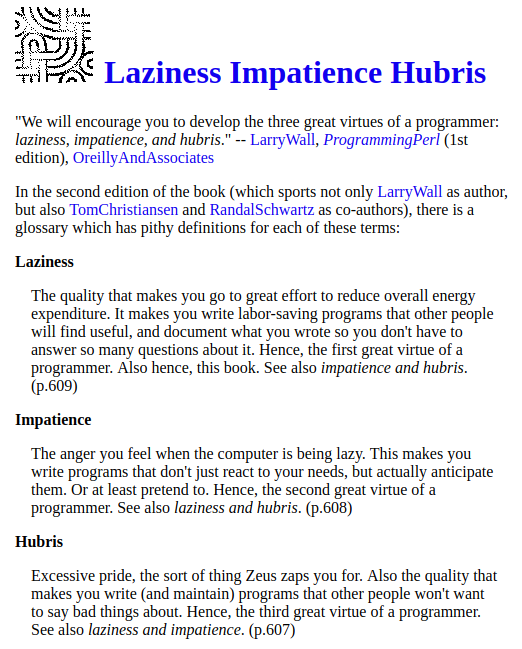
\includegraphics[width=1.0\textwidth]{figures/xunit/larry-wall.png}
\caption{优秀程序员的三大美德: 懒惰、缺乏耐心和傲慢}
 \label{fig:larry-wall}
\end{figure}

优秀的程序员总是设法寻找高效的工作方法,并将其成为工作的日常习惯。因为懒惰,程序员痛恨机械的重复工作,而追求程序自动实现;因为缺乏耐心,而追求程序行云流水;因为傲慢,而追求程序至善至美。

\subsubsection{重构神器}

\emph{实践\ascii{TDD},尽快变绿是当务之急}。我常习惯于在测试用例上方的匿名命名空间内,就近直接实现产品代码。如此加快通过测试用例的速度,及其避免在实现与测试之间来回跳转而分散注意力。

当测试通过后,应用重构将实现逐一搬迁至产品代码中。这时需要特别注意重构的习惯,不要立即\emph{剪切}实现,而应该使用\emph{复制}。当关键步骤完成时,都需要运行测试用例。直至从测试代码中搬迁完成所有相关实现至产品之中,最后再从测试代码中安全地删除。

这是重构的基本素养,不至于在重构之中慌了手脚,迷失自我。自信也是影响代码质量的关键因素,如果很长时间内未得到测试成功的反馈结果,自信指数自然下跌。相反地,如果每个微小的步骤都是成功的,正反馈必然促进信心指数上涨,使得编程成为一种乐趣,而不至于陷入一味调试的泥潭之中。

如上例所示,需要将特化实现的\ascii{run}实现重构为模板函数。第一步,在产品代码中新建文件\ascii{TestMethod.h},复制既有的\ascii{run}实现,创建一个新函数\ascii{runX},并将其重构为模板函数。

\begin{c++}[title={\ttfamily{重构: 搬迁实现}}]
// in test
void run(WasRun& self, void(WasRun::*method)()) {
  (self.*method)();
}

// in product
template <typename Fixture>
void runX(Fixture& self, void(Fixture::*method)()) {
  (self.*method)();
}
\end{c++}

第二步,搜索所有引用\ascii{run}函数的地方,逐一替换为\ascii{runX}。每替换一个,运行一遍测试用例;如果成功,立即执行\ascii{git add}。直至所有引用\ascii{run}的地方替换为\ascii{runX}。最后,再安全地删除既有的\ascii{run}函数。

第三步,运用\ascii{Alt + Shift + R}重命名\ascii{runX}为\ascii{run},确保通过测试。

\subsubsection{Git神器}

感谢\ascii{Linus}创造了\ascii{Linux}与\ascii{Git},让全世界的程序员得以享受编程的快乐。\ascii{TDD}精髓之一便是“小”,配合运用\ascii{Git},简直就是完美,避免不经意的错误而丢失代码。

养成经常性提交代码至\ascii{Git}库,是一种良好的编程习惯。在\ascii{TDD}的一个迭代循环中,每当编译通过,链接通过,测试通过,关键重构成功,都应立即执行\ascii{git add}。当设计重构至相对合理状态,最后执行\ascii{git commit}入库,完成一次\ascii{TDD}的闭环。

此外,借助于\ascii{Git},随时可以吃后悔药。当尝试某种重构设计时,没有达到预期效果,则可以轻松回到上一个稳定状态,重新开始尝试新的努力。以“重命名函数”的重构过程为例,讲述\ascii{Git}的操作。

\begin{enum}
  \eitem{新建一个函数;}
  \eitem{拷贝旧函数的实现至新函数;}
  \eitem{确保编译、测试通过,执行\code{git add};}  
  \eitem{删除旧函数的实现逻辑,转调新函数;}
  \eitem{确保编译、测试通过,执行\code{git add};}
  \eitem{对于每个引用旧函数的地方,重构引用新函数,确保编译、测试通过,执行\code{git add};}    
  \eitem{删除旧函数,确保编译、测试通过,执行\code{git commit}。}      
\end{enum}

\end{content}
\end{episode}

\subsection{自动实例}

\ascii{run}函数虽然已经泛化了,但是它仅仅实现了测试方法的间接调用,其职责也很鸡肋。再次深入分析客户现场,用户更期待能够直接执行\emph{测试方法},并不期望还要负责创建和维护相关的\emph{测试对象}。重构既有测试用例使其失败,使其\ascii{run}函数不再依赖于具体的测试对象。

\begin{diff}{test/mars/core/TestMethodSpec.cc}
\begin{minicpp}
#include <mars/core/TestMethod.h>
#include <gtest/gtest.h>

namespace {
  struct WasRun {
    bool wasRun = false;

    void testMethod() {
      wasRun = true;
    }
  };
}

TEST(WasRunSpec, make_sure_test_method_be_ran) {
  WasRun test;

  ASSERT_FALSE(test.wasRun);
  run(test, &WasRun::testMethod);
  ASSERT_TRUE(test.wasRun);
}
\end{minicpp}
\tcblower
\begin{minicpp}
#include <mars/core/TestMethod.h>
#include <gtest/gtest.h>

namespace {
  bool wasRun = false;

  struct WasRun {
    void testMethod() {
      wasRun = true;
    }
  };
}

TEST(WasRunSpec, make_sure_test_method_be_ran) {
  ASSERT_FALSE(wasRun);
  run(&WasRun::testMethod);
  ASSERT_TRUE(wasRun);
}
\end{minicpp}
\end{diff}

为了能够快速通过测试,泛化的\ascii{run}函数额外承担\emph{测试对象}创建和维护的职责。此处,\ascii{xUnit Mars}执行引擎与客户建立了一个隐式的契约关系:\emph{测试对象必须具有默认构造函数},否则编译失败。目前,这个契约已经在\ascii{xUnit}社区得到了一致的认可。

\begin{diff}{include/mars/core/TestMethod.h}
\begin{minicpp}
template <typename Fixture>
void run(Fixture& self, void(Fixture::*method)()) {
  (self.*method)();
}
\end{minicpp}
\tcblower
\begin{minicpp}
template <typename Fixture>
void run(void(Fixture::*method)()) {
  Fixture self;
  (self.*method)();
}
\end{minicpp}
\end{diff}

\subsection{类型别名}

不幸的是,在\ascii{run}实现中,其参数类型声明为\code{void(Fixture::*method)()},极其难于理解。一般地,对于指向成员函数的指针,常引入类型别名,提高其表达力。

\begin{diff}{include/mars/core/TestMethod.h}
\begin{minicpp}
template <typename Fixture>
void run(void(Fixture::*method)()) {
  Fixture self;
  (self.*method)();
}
\end{minicpp}
\tcblower
\begin{minicpp}
template <typename Fixture>
using TestMethod = void(Fixture::*)();

template <typename Fixture>
void run(TestMethod<Fixture> method) {
  Fixture self;
  (self.*method)();
}
\end{minicpp}
\end{diff}

\subsection{函数对象}

重构既有的测试用例,使其符合\ascii{OO}的调用风格。

\begin{diff}{test/mars/WasSucc.cc}
\begin{minicpp}
TEST(TestSuiteSpec, make_sure_test_method_be_ran) {
  auto test = &WasSucc::testMethod;

  ASSERT_FALSE(wasSucc);
  run(test);
  ASSERT_TRUE(wasSucc);
}
\end{minicpp}
\tcblower
\begin{minicpp}
TEST(TestSuiteSpec, make_sure_test_method_be_ran) {
  TestMethod<WasSucc> test(&WasSucc::testMethod);

  ASSERT_FALSE(wasSucc);
  test.run();
  ASSERT_TRUE(wasSucc);
}
\end{minicpp}
\end{diff}

为了通过测试,引入函数对象\ascii{TestMethod},将\ascii{run}搬迁成为\ascii{TestMethod}的成员函数。此时,\ascii{TestMethod}持有\emph{测试对象},并负责执行\emph{测试方法}。可以将\ascii{TestMethod}看做\emph{测试方法}的包装器,相对于普通的模板函数\ascii{run},\ascii{TestMethod}更具设计弹性的空间。

\begin{diff}{include/mars/core/TestMethod.h}
\begin{minicpp}
template <typename Fixture>
using TestMethod = void(Fixture::*)();

template <typename Fixture>
void run(TestMethod<Fixture> method) {
  Fixture self;
  (self.*method)();
}
\end{minicpp}
\tcblower
\begin{minicpp}
template <typename Fixture>
struct TestMethod {
private:
  using Method = void(Fixture::*)();

public:
  TestMethod(Method method)
    : method(method) {
  }

  void run() {
    (self.*method)();
  }

private:
  Fixture self;
  Method method;
};
\end{minicpp}
\end{diff}

\begin{episode}{TDD: 测试驱动开发}
\begin{content}

\ascii{TDD}是极限编程中重要的技术实践之一。\ascii{TDD}遵循\emph{测试先行,小步快走,尽快变绿,事后重构}的基本方法论。把握\ascii{TDD}动态变化过程,做到收放自如,需要长期编程实践的经验积累。

\ascii{TDD}基本素养讲究两个字:“小”和“快”。“小”体现在测试刚好失败,实现恰如其分,重构步骤粒度甚微。而“快”体现不在于编程速度,而在于“尽最小努力,最短时间,最快通过测试”。

如果步子迈得过大,则恢复测试时间间隔会变长,信心指数则会下降,自然影响软件质量,甚至拖延软件交付进度。

\subsubsection{TDD闭环}

如\refig{tdd-cycle}所示,在一轮\ascii{TDD}编程实践过程中,遵循三部曲的闭环操作:\ascii{“Red-Green-Refactor”}。每轮迭代之后,确保系统都处于一个相对合理的状态。

\begin{figure}[H]
\centering
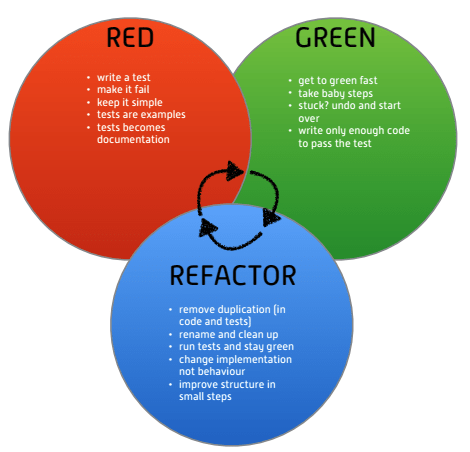
\includegraphics[width=0.8\textwidth]{figures/xunit/tdd-cycle.png}
\caption{TDD: 测试驱动开发}
 \label{fig:tdd-cycle}
\end{figure}

\subsubsection{TDD实现方法}

极限编程之父\ascii{Kent Beck}在经典著作\ascii{Test-Driven Development by Example}之中,介绍了三种基本的实现方法。

\begin{enum}
  \eitem{伪实现}
  \eitem{三角法}
  \eitem{显式实现}
\end{enum}

使用硬编码,伪装通过测试是一种最快速、最简单的实现方法。一旦通过测试,然后通过重构消除重复,以期待消除所有硬编码;或使用三角法,添加新的测试用例,驱动真实实现。

除非问题看起来并没有想象中那么简单,可以采取保守的策略也是恰当的。如果实现显而易见,完全可以绕开保守的\emph{伪实现}与\emph{三角法}。而在实际操作中,通过测试往往都比较简单,显式实现也是最常见的做法。在这种情况下,大可快速前进,不用处处敬小慎微。

\subsubsection{尽快变绿}

三种实现方法常常交替使用,虽然实现迥异,但殊途同归:以最小的努力,在最短的时间,通过测试,尽快变绿。实现过程中,尽量不要引入过度复杂的实现。例如,引入某种设计模式,重构既有的代码。

务必克服心中的恶魔,需要充分衡量成本收益比。如果引入设计较为笨重,通过测试遥遥无期,则应立即放弃;而如果引入设计显而易见,实施起来也比较容易操作,并带来一定设计的弹性,且不影响通过测试的整体进度,则可以有限接受。

\subsubsection{重构成为习惯}

一旦测试通过,务必重构既有的实现,让设计保持在目前最合理的状态。此刻,也需要克服心中的恶魔,不能做过度的设计。如果没有测试用例表达某个事件发生,则不要凭空臆想未来的世界会发生什么事情。

\subsubsection{出错后放慢脚步}

在最坏的情况下,测试在一段时间内尝试修复都以失败告终,则需要使用\ascii{Git}回退所有代码,使用更保守的\emph{伪实现}与\emph{三角法},尽快修复测试。

\subsubsection{TDD实现原则}

\ascii{Bob}大叔在其著作\ascii{Clean Code}中阐述了实践\ascii{TDD}的三个基本原则。

\begin{enum}
  \eitem{在编写不能通过的测试前,不可编写生产代码;}
  \eitem{只可编写刚好无法通过的测试,不能编译也算不通过;}
  \eitem{只可编写刚好足以通过当前失败测试的生产代码。}
\end{enum}

理解起来比较绕口,换一个等价的、较易理解的方式,可以表述为:

\begin{enum}
  \eitem{测试先行;}
  \eitem{测试失败;}
  \eitem{尽快变绿。}
\end{enum}

\subsubsection{TDD实现技巧}

实践\ascii{TDD}时,常需要规划和维护一个\ascii{TODO List}。将熟悉的,价值大,容易实现,高优先级的测试用例优先实现;而将不熟悉,价值小,不易实现,异常边界的测试用例依次排到后面,留待后续处理。

\begin{enum}
  \eitem{基本功能与异常场景;}  
  \eitem{高价值与现成果实;}
  \eitem{确定与不确定;}
  \eitem{整体优先与细节优先。}
\end{enum}

\end{content}
\end{episode}


\end{content}

